% debut d'un fichier latex standard
\documentclass[a4paper,12pt,twoside]{article}

% Pour les unités SI
\usepackage{siunitx}
% pour l'inclusion de figures en eps,pdf,jpg
\usepackage{graphicx}
% quelques symboles mathematiques en plus
\usepackage{amsmath}
% le tout en langue francaise
%\usepackage[english]{babel}
% on peut ecrire directement les caracteres avec l'accent
% a utiliser sur Linux/Windows
\usepackage[utf8]{inputenc}
\usepackage[T1]{fontenc}

% pour faire des systèmes d'équations
\usepackage{systeme}
\setcounter{tocdepth}{3} % Augmente le niveau affiché dans la table des matières

% a utiliser sur le Mac
%\usepackage[applemac]{inputenc}
% pour l'inclusion de links dans le document
\usepackage[colorlinks,bookmarks=false,linkcolor=blue,urlcolor=blue]{hyperref}
\usepackage{subcaption}
\paperheight=297mm
\paperwidth=210mm

\setlength{\textheight}{235mm}
\setlength{\topmargin}{-1.2cm} % pour centrer la page verticalement
%\setlength{\footskip}{5mm}
\setlength{\textwidth}{15cm}
\setlength{\oddsidemargin}{0.56cm}
\setlength{\evensidemargin}{0.56cm}

\pagestyle{plain}

% quelques abreviations utiles
\def \be {\begin{equation}}
\def \ee {\end{equation}}
\def \dd  {{\rm d}}

\newcommand{\mail}[1]{{\href{mailto:#1}{#1}}}
\newcommand{\ftplink}[1]{{\href{ftp://#1}{#1}}}
%
% latex SqueletteRapport.tex      % compile la source LaTeX
% xdvi SqueletteRapport.dvi &     % visualise le resultat
% dvips -t a4 -o SqueletteRapport.ps SqueletteRapport % produit un PostScript
% ps2pdf SqueletteRapport.ps      % convertit en pdf

% pdflatex SqueletteRapport.pdf    % compile et produit un pdf


% ======= Le document commence ici ======

\begin{document}
% Le titre, l'auteur et la date
\title{Exercise 3: Pendulum with a vertical excitation\\{\small Physique Numérique I}}
\date{\today}
\author{Delphine Martres et Damien Korber\\{\small \mail{delphine.martres@epfl.ch} et \mail{damien.korber@epfl.ch}}}
\maketitle
\tableofcontents % Table des matieres
\newpage % Si la toc est trop grande, voir ligne 19.
% Quelques options pour les espacements entre lignes, l'identation
% des nouveaux paragraphes, et l'espacement entre paragraphes
\baselineskip=16pt
\parindent=15pt
\parskip=5pt



%%%% ON COMMENCE A ECRIRE D'ICI

\section{Introduction}

\section{Analytical computations}
\subsection{Differential equation of the problem}
After some computations described in appendix \ref{ann:eq-diff}, equation \ref{eq:equa-diff} results.%TODO: Faire l'annexe en question.

\begin{equation}
	\ddot{\theta} = -\frac{\kappa}{m}\dot{\theta} - \frac{g}{L}\sin\theta
	\label{eq:equa-diff}
\end{equation}
where $\kappa$ is an air resistance coefficient, $m$ is the mass, $\theta$ is the angle of the pendulum, $g$ the mean gravity on earth and $L$ the length of the rod.

Equation \ref{eq:equa-diff} can also be written as equation \ref{eq:equa-diff-sys}, which is better for numerical computations.

\begin{equation}
	\frac{d}{dt}
	\begin{pmatrix}
		\theta \\ \dot{\theta}
	\end{pmatrix}
	= \begin{pmatrix}
	\dot{\theta} \\
		-\frac{\kappa}{m}\dot{\theta} - \frac{g}{L}\sin\theta
	\end{pmatrix}
	\label{eq:equa-diff-sys}
\end{equation}

\subsection{Mechanical energy and power of non-conservative forces in the frame of reference $R'$}
The only energy to consider is the kinetic energy of rotation, and the potential energy, as there is no translation.
The kinetic energy of rotation is given by $E_{c,r} = \frac{1}{2}I\omega^2$, where $I$ is the moment of inertia and $\omega$ the angular velocity.
The moment of inertia of a solid can be tough to compute for generic objects, but for a discrete number of masses, the moment of inertia is given by equation \ref{eq:moment-inertie}. \cite{ans:moment-inertie} %TODO: Ajouter à la bibliographie le livre de meca pour la formule de I.

\begin{equation}
	I = \sum_\alpha m_\alpha r_\alpha^2
	\label{eq:moment-inertie}
\end{equation}
where $m_\alpha$ is the mass and $r_\alpha$ is the distance between the origin considered and the mass.

In the case of the pendulum, it is quite trivial to compute.
The mass of rod of the pendulum is ignored, and the mass $m$ of the pendulum is condensed in a single point at a distance $L$ of the origin of $R'$.
The moment of inertie is the given by $I=mL^2$.\\ %TODO: J'ai pas trouvé de traduction de "point matériel".

The mechanical is then expressed as equation \ref{eq:emec}.

\begin{equation}
	E_m = \frac{1}{2}I\omega^2 - mgL\cos\theta =  \frac{mL^2}{2}\dot{\theta}^2 - mgL\cos\theta
	\label{eq:emec}
\end{equation}

Regarding the power, there is only one force to consider, the air resistance (or drag), because it is the only non-conservative one.
The power is expressed as $P = \mathbf{F}\cdot\mathbf{v}$, and the drag is defined as $\mathbf{f} = -\kappa\mathbf{v'}$ in this report, where $\mathbf{v'}$ is the speed in the frame of reference $R'$.
These vectors are given by:

\begin{align*}
	\mathbf{f} = 
	\begin{pmatrix}
		f\cos\theta \\
		f\sin\theta \\
		0
	\end{pmatrix}
	= \begin{pmatrix}
		f\cos\theta \\
		f\sin\theta \\
		0
	\end{pmatrix}
	\text{ and }
	\mathbf{v} =
	\begin{pmatrix}
		-v'\cos\theta \\
		-v'\sin\theta \\
		0
	\end{pmatrix}
	= \begin{pmatrix}
		-\dot{\theta}L\cos\theta \\
		-\dot{\theta}L\sin\theta \\
		0
	\end{pmatrix}
\end{align*}

The power of the drag is then given by equation \ref{eq:power}.
\begin{equation}
	P = \kappa\dot{\theta}^2 L^2
	\label{eq:power}
\end{equation}

\subsection{Solutions for little movements around equilibrium}
%TODO: à remplir
\section{Numerical computations}

\subsection{Little movements without excitation or air resistance}
In this section, no excitation or air resistance will be considered: $\kappa = 0$, $d = 0$.
The movements are small, and approximations are made: $\theta_0 = \num{d-6}$, $\dot{\theta}_0 = 0$.
The computations run for \SI{20}{\second}.

\subsubsection{Comparison between the analytical solution and the approximation of Stormer-Verlet method}
\begin{figure}[h]
\begin{subfigure}[t]{0.48\textwidth}
	\includegraphics[width=\textwidth]{graphs/a_traj_full.eps}
	\caption{Angle of the pendulum with respect to time, with a comparison between the Stormer-Verlet numerical method and the analytical solution.}
	\label{fig:a-traj-full}
\end{subfigure}
~
\begin{subfigure}[t]{0.48\textwidth}
	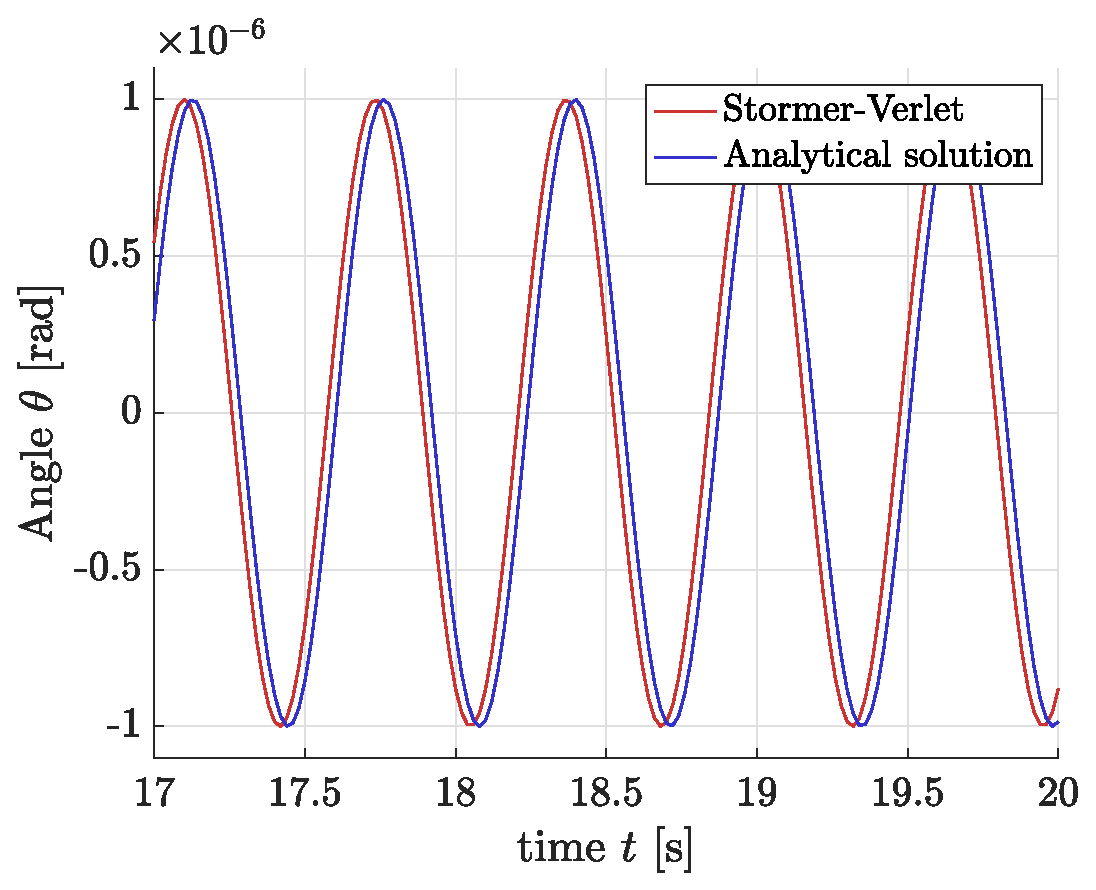
\includegraphics[width=\textwidth]{graphs/a_traj_zoomed.eps}
	\caption{Same plot as \ref{fig:a-traj-full}, with the beginning cropped out to get a better view of the small difference between the numerical and analytical solutions.}
	\label{fig:a-traj-zoomed}
\end{subfigure}
\caption{Angle of the pendulum with respect to time.}
\label{fig:a-traj}
\end{figure}

\subsubsection{Convergence study}

\subsubsection{Conservation of energy}

\subsection{Great movements}

\subsection{Resonant excitation}

\subsection{Parametric excitation}

\subsection{Poincaré section: chaos without air resistance}

\subsection{Pointcaré section: chaos with air resistance}

\end{document}
